\documentclass[tikz,border=5pt]{standalone}

\usepackage{pgfplots}
\pgfplotsset{compat=1.18}

\begin{document}

%------------------------------------------------
% Image 1: y = 2^x with emphasis at x = 1
%------------------------------------------------
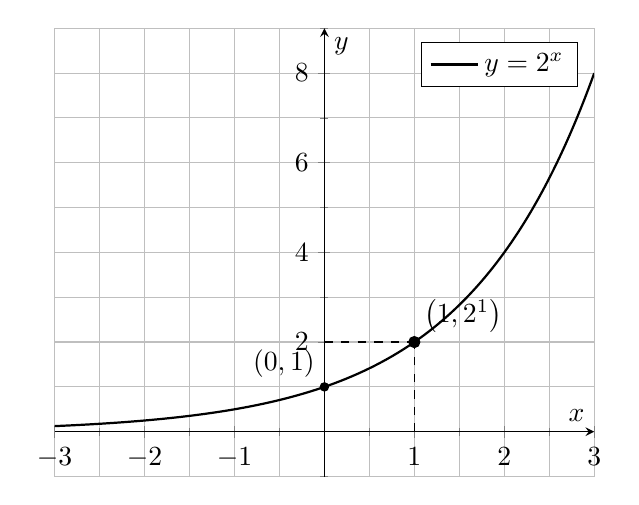
\begin{tikzpicture}
  \begin{axis}[
      axis lines = middle,
      xmin = -3, xmax = 3,
      ymin = -1, ymax = 9,
      samples = 200,
      xlabel = {$x$},
      ylabel = {$y$},
      grid = both,
      minor tick num = 1,
      domain = -3:3,
      legend style={at={(0.97,0.97)},anchor=north east},
    ]

    % Plot y = 2^x
    \addplot[thick] {2^x};
    \addlegendentry{$y = 2^x$}

    % Emphasize the point (1, 2)
    \addplot[
      only marks,
      mark=*,
      mark size=2pt
    ] coordinates {(1,2)};

    % Dashed helper lines to the axes
    \addplot[dashed] coordinates {(1,0) (1,2)};
    \addplot[dashed] coordinates {(0,2) (1,2)};

    % Label the point
    \node[above right] at (axis cs:1,2)
      {$\big(1,2^1\big)$};

    % Label the y-intercept at x=0 (optional)
    \addplot[
      only marks,
      mark=*,
      mark size=1.5pt
    ] coordinates {(0,1)};
    \node[above left] at (axis cs:0,1)
      {$(0,1)$};

  \end{axis}
\end{tikzpicture}

\newpage

%------------------------------------------------
% Image 2: y = ln(x) with emphasis at x = 1
%------------------------------------------------
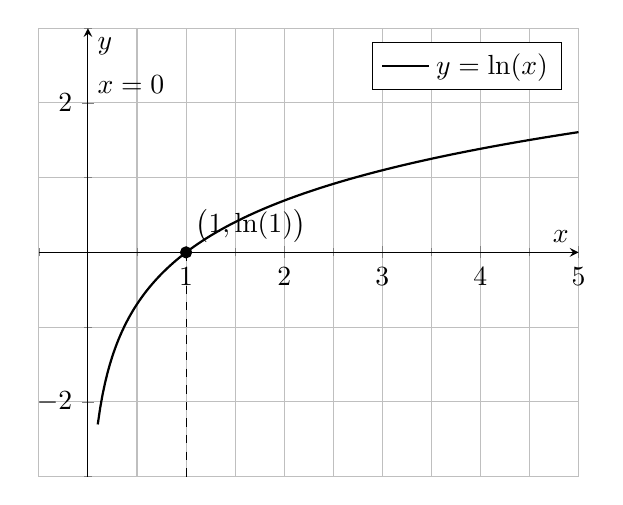
\begin{tikzpicture}
  \begin{axis}[
      axis lines = middle,
      xmin = -0.5, xmax = 5,
      ymin = -3,   ymax = 3,
      samples = 200,
      xlabel = {$x$},
      ylabel = {$y$},
      grid = both,
      minor tick num = 1,
      domain = 0.1:5,
      legend style={at={(0.97,0.97)},anchor=north east},
    ]

    % Plot y = ln(x)
    \addplot[thick, domain=0.1:5] {ln(x)};
    \addlegendentry{$y = \ln(x)$}

    % Vertical asymptote x=0 (optional)
    \addplot[dashed] coordinates {(0,-3) (0,3)};
    \node[below right] at (axis cs:0,2.5)
      {$x=0$};

    % Emphasize the point (1,0)
    \addplot[
      only marks,
      mark=*,
      mark size=2pt
    ] coordinates {(1,0)};

    % Dashed helper lines to the axes
    \addplot[dashed] coordinates {(1,0) (1,-3)};
    \addplot[dashed] coordinates {(0,0) (1,0)};

    % Label the point
    \node[above right] at (axis cs:1,0)
      {$\big(1,\ln(1)\big)$};

  \end{axis}
\end{tikzpicture}

\end{document}
